\documentclass[border=6pt]{standalone}
\usepackage{tikz}
\usetikzlibrary{arrows.meta,positioning,calc,shapes.geometric,fit,backgrounds,patterns,matrix,decorations.pathreplacing}
\begin{document}
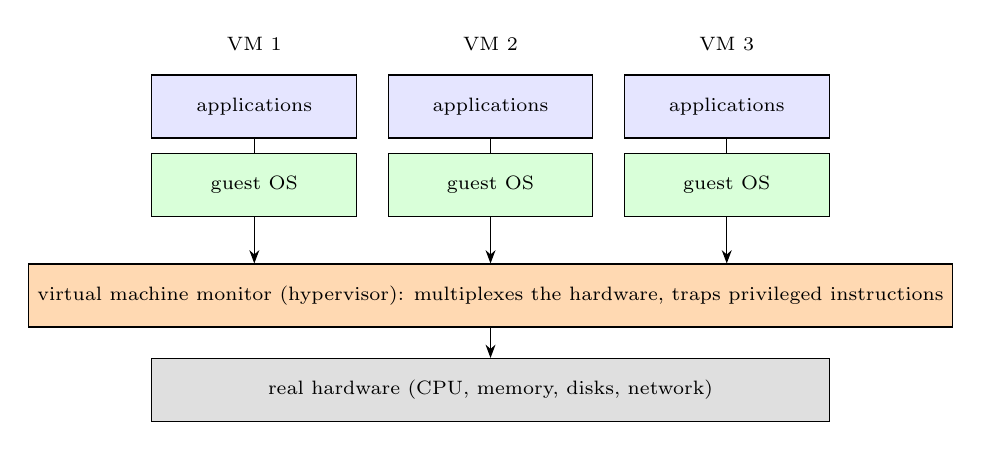
\begin{tikzpicture}[>=Stealth,font=\small]
\tikzstyle{b}=[draw,align=center,font=\scriptsize,minimum height=0.8cm]
\foreach \i/\n in {0/{VM 1},1/{VM 2},2/{VM 3}} { \node[b,fill=blue!10,minimum width=2.6cm] (a\i) at (\i*3.0,2.2) {applications}; \node[b,fill=green!15,minimum width=2.6cm] (g\i) at (\i*3.0,1.2) {guest OS}; \node[font=\scriptsize] at (\i*3.0,3.0) {\n}; \draw (a\i) -- (g\i); }
\node[b,fill=orange!30,minimum width=8.6cm] (vmm) at (3.0,-0.2) {virtual machine monitor (hypervisor): multiplexes the hardware, traps privileged instructions};
\node[b,fill=gray!25,minimum width=8.6cm] (hw) at (3.0,-1.4) {real hardware (CPU, memory, disks, network)};
\draw[->] (g0.south) -- (g0.south |- vmm.north); \draw[->] (g1.south) -- (g1.south |- vmm.north); \draw[->] (g2.south) -- (g2.south |- vmm.north);
\draw[->] (vmm) -- (hw);
\end{tikzpicture}
\end{document}
